%% ---------------------------------------------------------------------------------------------------------------------

\chapter{Analysis of Security Problems with Unsafe}\label{ch:unsafe-security-problems}

This chapter presents an in-depth security analysis of possible consequences and vulnerabilities that can be caused by
misuses of the \unsafe{} \acrshort{API}.
It is organized into three main areas of danger.
First, buffer overflow bugs and their consequences including code injection and information leak vulnerabilities are
shown.
The following section is about incorrect conversion between slices and strings, which among others can lead to
\textit{use-after-free} bugs on multiple ways.
Finally, the dangers of conversions between types with architecture-dependent sizes are discussed.

\begin{figure}[htp!]
    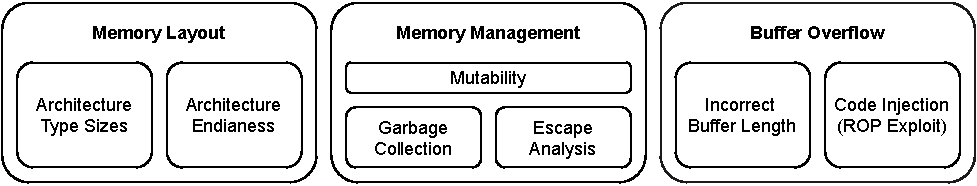
\includegraphics[width=\textwidth]{assets/figures/chapter3/outline3.pdf}
    \caption{Role of chapter 3 in the thesis outline}
    \label{fig:outline3}
\end{figure}



%% ---------------------------------------------------------------------------------------------------------------------

\section{Architecture-Dependent Types}\label{sec:unsafe-security-problems:architecture-dependent-types}

The third area of possible vulnerabilities concerns types that have a different size or alignment on different
architectures.
A feature of Go is portability between different platforms.
The same source code can usually be compiled for many different architectures without any changes in its behavior.
However, this is only true as long as the \unsafe{} \acrshort{API} is not used.
Since \unsafe{} code allows direct conversion between arbitrary types, there can be inconsistencies between the sizes
and alignments of structure fields on different architectures.
An example of this is shown in Listing~\ref{lst:architecture-dependent-types-cast}.

\begin{lstlisting}[language=Golang, label=lst:architecture-dependent-types-cast, caption=Incorrect cast between architecture-dependent types]
func main() {
    bytesResult := GetBytes()
    fmt.Printf("main: \%s\n", bytesResult) // expected (but failed) stdout is "abcdefgh
}

func GetBytes() []byte {
    reader := bufio.NewReader(strings.NewReader("abcdefgh"))
    s, _ := reader.ReadString('\n')
    out := StringToBytes(s)
    fmt.Printf("GetBytes: \%s\n", out) // expected stdout is "abcdefgh"
    return out
}
\end{lstlisting}

There are two structure types declared, \textit{PinkStruct} (Lines~1--4) and \textit{VioletStruct} (Lines~5--8), both of
which have two fields \textit{A} and \textit{B}.
While field \textit{B} has the same type (\textit{uint8}) in both types, field \textit{A} is of type \textit{int}
(Line~2) and \textit{int64} (Line~6), respectively.
An instance of \textit{PinkStruct} is created in Line~11, which is then converted to \textit{VioletStruct} in Line~12.
This is however only a valid operation if \textit{int} and \textit{int64} share the same size and alignment.

This is true only for 64-bit platforms like \textit{amd64}.
If the code is run on such an architecture, the conversion works fine and the field values in the resulting variable
\textit{violet} are as expected.
In contrast, if the code is run on an architecture where \textit{int} and \textit{int64} have different size or
alignment, then the values of \textit{violet} are undefined.
This is the case for example when the code is run on a 32-bit platform like \textit{i386}.
When the structure definitions are not placed directly next to each other but in separate files, packages, or even
modules, then spotting the difference between the incompatible structs is much harder.
On top of that, the bug might never occur in testing but only on specific platforms that get used in production.
Possible consequences of a bug like this depend on how the resulting struct is used in the remainder of the program.
If data gets written to it, it changes invalid memory which can lead to a code injection vulnerability, and if it is
passed as output it could create an information leak vulnerability.

On top of other field sizes, there could also be a different endianess on some architecture.
In this case, using a direct cast using the \unsafe{} \acrshort{API} is not aware of possible changes of the byte order,
for example incoming network data and data stored in the memory could be represented as big and little endians and cause
a mismatch.
When such data is stored as the length of a slice, the number could be misinterpreted and thus a slice with a wrong
length could be created.
This in term causes a buffer overflow vulnerability with the consequences discussed earlier.

\begin{insight}
    Different type sizes and endianess on various architectures, used with direct conversions through
    \textit{unsafe.Pointer}, can cause invalid memory access such as buffer overflows.
\end{insight}


%% ---------------------------------------------------------------------------------------------------------------------

\section{Incorrect Slice and String Casts}\label{sec:unsafe-security-problems:slice-casts}

The second main area of danger with \unsafe{} usages is focused around the conversion of slices and string of different
types.


%% ---------------------------------------------------------------------------------------------------------------------

\subsection{Implicit Read-Only}\label{subsec:unsafe-security-problems:slice-casts:read-only}

Listing~\ref{lst:string-to-bytes} shows a common \unsafe{} usage pattern that takes a string argument and converts it
into a slice of bytes without allocating additional memory.
This allows to access the raw bytes contained in the string in an efficient manner.

\begin{lstlisting}[language=Golang, label=lst:string-to-bytes, caption=Conversion from \textit{string} to \textit{[]byte} using \unsafe{}]
func StringToBytes(s string) []byte {
    strHeader := (*reflect.StringHeader)(unsafe.Pointer(&s))
    bytesHeader := reflect.SliceHeader{
        Data: strHeader.Data,
        Cap:  strHeader.Len,
        Len:  strHeader.Len,
    }
    return *(*[]byte)(unsafe.Pointer(&bytesHeader))
}
\end{lstlisting}

First, the string is converted into the \textit{reflect.StringHeader} representation in Line~2.
Then, a slice header is created as a composite literal and the reference to the underlying data array and length
information are copied from the string header (Lines~3--7).
The capacity is set to the same value as the length, as it would be in a slice that uses the full allocated capacity.
Finally, the slice header is converted into an actual \textit{[]byte} slice which is returned (Line~8).

There are three not obvious but very dangerous problems that come with this type of slice creation, which are described
in this and the following two subsections.
The first is that the resulting slice is implicitly read-only.

Regularly, slices in Go are mutable and strings are not.
The reason for this is that slices are created dynamically, with their backing array usually placed on the heap, while
strings are mostly constants that are part of the constant data or text section of the program binary after compilation.
The actual string characters, to which the data reference in the string header will be pointing, are therefore usually
located on a memory page that is not writable, and mutating the string would thus make the program receive a
segmentation fault signal from the operating system.
To statically prevent this at compilation time, strings are always immutable in Go, while slices are mutable.
If a developer writes code that changes parts of a string in-place, then the compiler will not accept the code and thus
prevent the possible segmentation fault.

In contrast, slices are mutable, and thus so is the slice returned by the \textit{StringToBytes} function in
Listing~\ref{lst:string-to-bytes}.
Code that changes the resulting slice will be accepted by the compiler because it is not able to infer its connection to
a former string.
However, since the slice uses the same underlying data array as the original string used to do, the data is still
potentially located within read-only memory, and modifying it will crash the program.
It is only implicitly read-only, but the runtime is not aware of it.
While this first problem of the conversion pattern does not cause a direct security vulnerability, it underlines that
there are many consequences of using the \unsafe{} \acrshort{API} that are not obvious.
Although it is possible in theory to manually ensure that no usages of the \textit{StringToBytes} function modify the
slice it returns, in practice it is very hard to do so, especially if new developers join the project after time and
start using the function without having all possible consequences in mind.


%% ---------------------------------------------------------------------------------------------------------------------

\subsection{GC Race Use-After-Free}\label{subsec:unsafe-security-problems:slice-casts:gc-race}

The second problem caused by the conversion shown in Listing~\ref{lst:string-to-bytes} is a \textit{use-after-free} bug
caused by a race condition involving the garbage collector (\acrshort{GC}) used by Go.

The \acrshort{GC} treats all pointer types and the special \textit{Data} field of actual slices and strings as reference
types.
Importantly though, it does not treat normal \textit{uintptr} values as references although they contain addresses.
This means that converting a \textit{uintptr} value to an \textit{unsafe.Pointer} value is an invalid and dangerous
operation.
If the \textit{GC} runs while the pointer has not been constructed, then it does not mark the value at the address
stored in the \textit{uintptr} value as live and thus frees the memory.
Creating an \textit{unsafe.Pointer} from this address therefore creates a potentially dangling pointer because it points
to memory that has been freed.
This is a \textit{use-after-free} bug.

The conversion pattern between strings and slices shown in Listing~\ref{lst:string-to-bytes} contains exactly this bug.
The \textit{Data} field of the \textit{reflect.SliceHeader} structure created in Line~3 is of type \textit{uintptr}, and
since the header value is not derived by cast from a real slice it does not benefit from the special case built into the
Go runtime that treats \textit{uintptr} references that are part of slice and strings as references, too.
Specifically, the problem is that the slice header has been constructed as a composite literal.
Therefore, after Line~7 the \textit{bytesHeader} variable effectively becomes a plain \textit{uintptr} value, and the
original string \textit{s} is not used any longer.
However, at this point there is no real slice created yet as this happens net earlier than in Line~8.
The underlying data array of the string \textit{s} is therefore not a live value as far as the \acrshort{GC} is
concerned.

\begin{figure}[!t]
    \vspace{2mm}
    \centering
    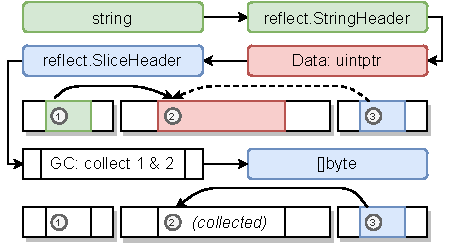
\includegraphics[width=0.4\textwidth]{gfx/figures/gcrace-vuln.pdf}
    %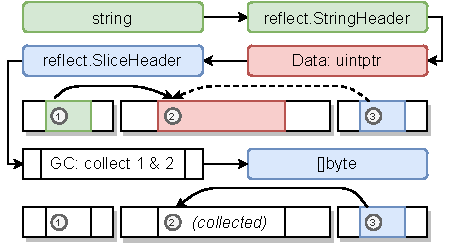
\includegraphics[width=0.48\textwidth]{gfx/figures/gcrace-vuln.pdf}
    \caption{GC race and escape analysis flaw}
    \label{fig:gcrace-vuln}
    \vspace{-8pt}
\end{figure}


If the \acrshort{GC} runs at the wrong time, the underlying data array used in the slice might have already been
collected by the time the resulting slice is created.
This is possible because since the \acrshort{GC} runs concurrently to the application logic, it can trigger at any time.
This is especially true if the Go program has several threads that all contribute to the heap usage.
Figure~\ref{fig:gcrace-vuln} illustrates the vulnerability.
The green boxes show the original string value and its header, which is represented at position 1 in the memory schema.
The reference to the underlying data of the string and resulting slice is shown in red at memory position 2.
Then the slice header is created, which is colored blue and located at position 3 in the memory.
References indicated by arrows are strong if the arrow is continuous, like the reference the string header has, and
weak if the arrow is dashed, like the new slice header has.
Then, after the \textit{GC} runs, there is only the resulting bytes slice left, which is also shown in blue.
It now has a strong reference to the underlying data array (at position 2), but since the \acrshort{GC} has already run
while there was only a weak reference to it, the data has been collected.
The resulting bytes slice is now a dangling pointer into the former string data in memory, and the
\textit{use-after-free} bug is complete.

A common variation to this insecure casting pattern is to omit storing the slice header that is created as a composite
literal in a variable and instead casting it into the resulting slice value within the same statement, as is shown in
Listing~\ref{lst:string-to-bytes-1statement}.

\begin{lstlisting}[language=Golang, label=lst:string-to-bytes-1statement, caption=Unsafe slice cast in one single statement]
strHeader := (*reflect.StringHeader)(unsafe.Pointer(&s))
return *(*[]byte)(unsafe.Pointer(&reflect.SliceHeader{
    Data: strHeader.Data,
    Cap:  strHeader.Len,
    Len:  strHeader.Len,
}))
\end{lstlisting}

This does however not affect the bugs and vulnerabilities shown in this
Section~\ref{sec:unsafe-security-problems:slice-casts}.
In fact, the assembly that the code gets compiled to is exactly the same for both versions in
Listings~\ref{lst:string-to-bytes} and~\ref{lst:string-to-bytes-1statement}.
Even if the assembly would be different, performing the creation of a slice header as a composite literal and casting it
to an actual slice in the same statement would still not avoid creating a plain \textit{uintptr} reference to the
underlying data array as far as the \acrshort{GC} is concerned.
This is because the \acrshort{GC} concurrency is at the level of machine instructions, not statements in the Go source
code.


%% ---------------------------------------------------------------------------------------------------------------------

\subsection{Escape Analysis Use-After-Free}\label{subsec:unsafe-security-problems:slice-casts:escape-analysis}

The third problem that comes with the incorrect construction of a new slice shown in Listing~\ref{lst:string-to-bytes}
in the previous section is that the Go compiler's escape analysis (\acrshort{EA}) algorithm fails.

The insecure string to slice conversion shown in Listing~\ref{lst:string-to-bytes} breaks the \acrshort{EA}.
This is because for a similar reason to the \acrshort{GC}, it misses the connection between the string parameter and
the slice return value.
Listing~\ref{lst:escape-analysis-flaw} shows a proof of concept of this problem.

\begin{lstlisting}[float=tp, language=Golang, label=lst:escape-analysis-flaw, caption=Escape analysis flaw proof of concept]
func main() {
    bytesResult := GetBytes()
    // expected stdout is "abcdefgh"
    // actual output is random invalid data
    fmt.Printf("main: %s\n", bytesResult)
}

func GetBytes() []byte {
    reader := bufio.NewReader(strings.NewReader("abcdefgh"))
    s, _ := reader.ReadString('\n')
    out := StringToBytes(s)
    // expected stdout is "abcdefgh"
    // actual output is "abcdefgh"
    fmt.Printf("GetBytes: %s\n", out)
    return out
}
\end{lstlisting}

In the function \textit{GetBytes}, a string variable \textit{s} is created by reading a string through a buffered
reader (Lines~9--10).
It is necessary to use the reader instead of a string literal, because with a literal the effects of the vulnerability
would not be visible.
This is however no restriction to the proof of concept.
Creating the string from a reader is similar to accepting dynamic user input.
Next, the string is converted to a byte slice using the insecure \textit{StringToBytes} function in Line~11.
Printing the resulting slice in Line~14 then yields the expected output equal to the original string, which is
\textit{abcdefgh}.
Finally, the slice is returned to the caller function, which in this case is the \textit{main} function in Line~2.
The slice is printed again in the \textit{main} function in Line~5, and while the expected output would be identical,
this time invalid, random data is printed.

The reason for this is that when the Go \acrshort{EA} algorithm determines where to allocate the string \textit{s} in
the \textit{GetBytes} function, it sees that \textit{s} is passed to the \textit{StringToBytes} function and therefore
transitively analyzes that function.
Within that function, \textit{s} is used in a cast to the \textit{strHeader} variable in Line~2 of
Listing~\ref{lst:string-to-bytes}, then that is used to construct the \textit{bytesHeader} variable, but at this point
there no further references to the underlying data array of \textit{s} because both \textit{s} and
\textit{strHeader} are not used further in the function.
Similarly to the \acrshort{GC} mark algorithm, the \textit{Data uintptr} field would only be treated as a reference with
respect to escape analysis if the slice header had been created by cast from an actual slice.
Therefore, the \acrshort{EA} determines that \textit{s} does not escape in \textit{StringToBytes}, and since it is not
used any longer in \textit{GetBytes}, it does not escape at all and is placed on the stack of the \textit{GetBytes}
function.
The \textit{EA} algorithm fails to detect that there is a reference to parts of the string \textit{s} stored in the
\textit{out} variable, which obviously escapes as it is returned.

Printing the \textit{out} slice in Line~15 works because the stack of the \textit{GetBytes} function is still there at
this point.
However, when the function returns the stack frame is removed, and thus \textit{bytesResult} in Line~2 has become a
dangling pointer into the former stack of \textit{GetBytes}.
This is a \textit{use-after-free} bug because that memory can and probably will be reused at that point.
The print statement in Line~5 outputs invalid data for this reason.
If the \textit{main} function would modify the contents of the \textit{bytesResult} slice, it would change arbitrary
memory, with possible consequences such as information leaks or code injection.

\begin{insight}
    \todo{Write insight}
\end{insight}


%% ---------------------------------------------------------------------------------------------------------------------

\section{Buffer Overflow Vulnerabilities}\label{sec:unsafe-security-problems:buffer-overflow}

The first main area of possible vulnerabilities in the context of the \unsafe{} \acrshort{API} are buffer overflows.
They are a rather common and dangerous problem with traditional systems programming languages like C, accounting for
many of the most severe security vulnerabilities~\cite{larochelle2001} \jl{second citation}.
When \unsafe{} code is used in Go, the safety measures provided by the language described in
Section~\ref{sec:background:memory-safety-layout} are circumvented.
Therefore, buffer overflows can happen just as well in that case.


%% ---------------------------------------------------------------------------------------------------------------------

\subsection{Incompatible Types}\label{subsec:unsafe-security-problems:slice-casts:incompatible-types}

Converting slices to strings and vice versa can be done simply by casting them, however this will cause the Go runtime
to allocate a new slice or string for the resulting value.
To improve efficiency by reusing the underlying data and only reinterpret it as data of a new type, it is possible to
use the \unsafe{} \acrshort{API} for an in-place cast.
Since the fields in the header structures shown in Listing~\ref{lst:reflect-header-types} are different in the presence
of the \textit{Cap} field, this is however only valid for conversions from slices to string.
In that case, the resulting string header, which shares the same location in memory with the original slice header, will
reuse the reference to the underlying data array as well as the length, and since the string header structure does not
contain any more fields the capacity information will remain in adjacent, unused memory.

In contrast, when converting a string to a slice directly, the source header structure is too short.
The resulting slice header will use correct values for its data reference and length, but the capacity field will
contain whatever is located in memory directly after the original string header.

% k8s.io/apiserver/pkg/authentication/token/cache/cached\_token\_authenticator.go:235

\begin{lstlisting}[language=Golang, label=lst:unsafe-string-to-bytes-direct, caption=Incorrect direct cast between string and slice]
// toBytes performs unholy acts to avoid allocations
func toBytes(s string) []byte {
    return *(*[]byte)(unsafe.Pointer(&s))
}
\end{lstlisting}

The resulting slice with random data in its capacity field is dangerous to use.
Operations that read from a slice, like using it in a loop to iterate over its contents, mostly only use the data
reference and length.
However, any action on the slice that uses the capacity, like taking subslices from it or appending data, is undefined
and can therefore become a security vulnerability.
There is an instance of this incorrect cast in the \textit{k8s.io/apiserver} package that is part of the
\textit{Kubernetes} project, showing a conversoin from \textit{string} to \textit{[]byte}.
It is shown in Listing~\ref{lst:unsafe-string-to-bytes-direct}.


%% ---------------------------------------------------------------------------------------------------------------------

\subsection{Incorrect Length Information}\label{subsec:unsafe-security-problems:slice-casts:incorrect-length}

A second possible misuse in the context of slice conversions is an incorrect length value set in the slice header.
This can happen quickly if the length information is calculated dynamically, especially if the user-supplied input data
is used to deduce the resulting value.
An example of such a bug is shown in Listing~\ref{lst:go-fuse-bug}.
It is taken from the \textit{hanwen/go-fuse} library\footnote{\url{https://github.com/hanwen/go-fuse}}, a Go
implementation of the server specification used for the userspace filesystem (\acrshort{FUSE}) available for
Linux~\footnote{\url{https://www.kernel.org/doc/html/latest/filesystems/fuse.html}}.
We already submitted a patch for this bug to the authors.

% github.com/hanwen/go-fuse fuse/opcode.go:299

\begin{lstlisting}[language=Golang, label=lst:go-fuse-bug, caption=Incorrect slice length bug in the \textit{hanwen/go-fuse} library]
func doBatchForget(server *Server, req *request) {
    in := (*_BatchForgetIn)(req.inData)
    wantBytes := uintptr(in.Count) * unsafe.Sizeof(_ForgetOne{})

    if uintptr(len(req.arg)) < wantBytes {
        // We have no return value to complain, so log an error.
        log.Printf("Too few bytes for batch forget.",
                   len(req.arg), wantBytes, in.Count)
    }

    h := &reflect.SliceHeader{
        Data: uintptr(unsafe.Pointer(&req.arg[0])),
        Len:  int(in.Count),
        Cap:  int(in.Count),
    }
    forgets := *(*[]_ForgetOne)(unsafe.Pointer(h))
    // ...
}
\end{lstlisting}

\acrshort{FUSE} uses a client / server architecture where filesystem implementations present a server that handles
requests from a specific kernel module.
The kernel module acts like a regular filesystem driver, but instead of executing operations in kernel space, it
forwards them to the user space \acrshort{FUSE} server.
Communication is done through the \textit{/dev/fuse} device node.
The listing shows a part of the \textit{doBatchForget} function, which is used to clear files, identified by their inode
number, from a cache that the filesystem might have.
\textit{go-fuse} is designed in a way that incoming data from the \textit{/dev/fuse} node is passed to handler functions
as byte slices (\textit{req.inData} and \textit{req.arg} in Lines~2 and~5) containing the raw, serialized request.
The handler function then casts the data into a suitable structure to access individual fields.
In this case, the request is converted into an instance of the \textit{\_BatchForgetIn} type (Line~2), which provides
access to the number of inodes to forget that are contained in the batch request through the \textit{in.Count} field
(Line~3).
The individual forget messages in serialized and concatenated form are available through the \textit{req.arg} array, so
to access them a new slice is created by defining its slice header from scratch (Lines~11--15).
The created slice uses the incoming request data containing the forget messages (\textit{req.arg}, Line~12) as its
underlying data array and the number of messages (\textit{in.Count}) both as length and capacity (Lines~13 and~14).

Since the \textit{in.Count} field is supplied as part of the request sent to the library, it can be controlled by an
attacker if they manage to conduct a man-in-the-middle attack and change the request for a malicious
one.
If the length is greater than the actual available number of data bytes, then the resulting \textit{forgets} slice
(Line~16) will read additional data after the end of the actual batch forgets request.
Depending of the concrete operation to forget inodes from a local cache, this could have severe consequences with
respect to security.
To prevent this from happening, the authors intended to check the length of the available data in Line~5, and if there
are too few bytes for the alleged number of forget requests, then the method should not proceed.
However, as the listing shows there is no actual code to stop further execution of the method, instead there is only a
log message noting that there was a malformed request with too few bytes available (Lines~7--8).
A proof-of-concept implementation of a potential attacker showed that the method actually reads invalid memory data
located after the request data.
In this case, a simple \textit{return} statement after Line~8 would have prevented this bug.


%%% ---------------------------------------------------------------------------------------------------------------------
%
%\subsection{Information Leak}\label{subsec:unsafe-security-problems:buffer-overflow:information-leak}
%
%Go uses a strict type system that encodes the buffer length in the type information.
%This prevents most buffer overflow vulnerabilities at compile time because the compiler can detect whether a given
%buffer will be large enough to store the data that gets written to it, as described in
%Section~\ref{sec:background:memory-safety-layout}.
%However, this safety measure is circumvented when the \unsafe{} \acrshort{API} is used in Go.
%Using direct casts through the \textit{unsafe.Pointer} type, it is possible to convert between buffers of different
%sizes.
%Listing~\ref{lst:information-leak} shows such a situation.
%
%\begin{lstlisting}[language=Golang, label=lst:information-leak, caption=Buffer information leak proof of concept]
func main() {
    harmlessData := [4]byte{'A', 'A', 'A', 'A'}
    secret := [6]byte{'s', 'e', 'c', 'r', 'e', 't'}
    var leakingInformation = (*[10]byte)(unsafe.Pointer(&harmlessData[0]))
    fmt.Println(string((*leakingInformation)[:]))
}
\end{lstlisting}
%
%In Line~2, a buffer of size four bytes called \textit{harmlessBuffer} is initialized with data.
%Then, Line~2 declares a buffer containing a secret value, which should stay internal to the application.
%Using the \unsafe{} \acrshort{API}, the \textit{harmlessBuffer} is then converted to a have a new length of ten bytes,
%although there is no reallocation (Line~4).
%The resulting buffer is finally printed (Line~5), which outputs not only the harmless four bytes, but also the secret.
%The secret data could for example be a cryptographic private key or password information.
%Therefore, this bug has created an information leak vulnerability.
%
%To motivate a situation where this bug can have serious consequences,
%Figure~\ref{fig:information-leak-threat-model-protocol} shows the specification of a simple client / server
%communication protocol.
%Both request and response types contain a version and message type field as well as a buffer for message-specific,
%serialized data of length 512 bytes.
%
%\begin{figure}[htp!]
    %\vspace{2mm}
    \centering
    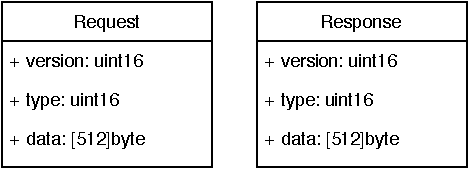
\includegraphics[width=0.5\textwidth]{assets/figures/chapter3/information-leak-threat-model-protocol.pdf}
    \caption{Example protocol to motivate threat model for unsafe cast}
    \label{fig:information-leak-threat-model-protocol}
    %\vspace{-10pt}
\end{figure}

%
%If the client or server handling these messages uses the \unsafe{} \acrshort{API} to convert the serialized data to a
%specific data structure, then the field lengths must match.
%Imagine a company where two different teams are working on the client and server, respectively, and they printed the
%protocol diagrams to hang them on the wall when the specification was decided.
%A developer in one of the teams could easily miss the announcement of a protocol change that affects the buffer size,
%and when they write incorrect code based on the outdated information on the printed diagram, the mistake could become
%unnoticed in code review due to the same reason, a reviewer who looks at the protocol diagram in the team room.


%% ---------------------------------------------------------------------------------------------------------------------

\subsection{Code Injection using ROP}\label{subsec:unsafe-security-problems:buffer-overflow:code-flow-redirection}

To create a classic input-based buffer overflow vulnerability, a byte slice with a length of 512 bytes is initializated,
but backed up with an underlying, much shorter byte buffer of only eight bytes.
Slices can be created using a cast from the \textit{reflect.SliceHeader} type which reflects the internal slice
irepresentation.
This is done in Lines~4 to~6 of Listing~\ref{lst:buffer-overflow}.

\begin{lstlisting}[language=Golang, label=lst:buffer-overflow, caption=Buffer overflow leading to code flow redirection]
func main() {
    harmlessData := [8]byte{'A', 'A', 'A', 'A', 'A', 'A', 'A', 'A'}

    confusedSlice := make([]byte, 512)
    sliceHeader := (*reflect.SliceHeader)(unsafe.Pointer(&confusedSlice))
    sliceHeader.Data = uintptr(unsafe.Pointer(&(harmlessData[0])))

    _, _ = bufio.NewReader(os.Stdin).Read(confusedSlice)
}
\end{lstlisting}


Then, a reader is used to read input data into this malicious slice in Line~8.
Since it has a length of 512 bytes, the function reads up to this many bytes, however since the actual data array used
by the slice is much shorter, this will overflow into the memory behind the data array.
In this case, the \textit{harmlessData} array is created on the stack of the function, which means it is vulnerable to
buffer overflow exploits as described in Section~\ref{sec:background:memory-safety-layout}.
An attacker can use this vulnerability to redirect the code flow by carefully crafting the input data such that the
saved return instruction pointer on the stack is overwritten with the address of a function of the attacker's choice.
To find the needed amount of padding before the address in the input data, as well as to find the target function's
address, the attacker can use a debugger such as \textit{GDB}.

A threat model for this kind of vulnerability would be an application that, similarly to the threat model described in
Section~\ref{subsec:unsafe-security-problems:buffer-overflow:information-leak}, uses a client server model, but this
time with a length information indicating how many bytes are sent within a variable-length data section as part of the
protocol.
If such a length field is used to construct a slice in the way shown in Listing~\ref{lst:buffer-overflow}, then an
attacker can control the resulting slice length and potentially exploit this bug to redirect to arbitrary code within
the binary.

Going a step further, this subsection shows how the same bug shown in the previous section in
Listing~\ref{lst:buffer-overflow} can be used with return-oriented programming (\acrshort{ROP}) to create a code
injection exploit.
A strategy to exploit a buffer overflow to achieve code injection using \acrshort{ROP} is to use the \textit{mprotect}
and \textit{read} system calls.
A system call, or syscall, is a function provided by the operating system which can be executed using the
\textit{syscall} machine instruction.
The processor registers control which syscall gets executed and which parameters it receives.
Therefore, an attacker only needs \acrshort{ROP} gadgets to control the contents of the registers, as well as to trigger
the syscall.
Using the \textit{mprotect} call, the attacker can set a memory area of their choice to have both writable and
executable flags, for example the heap area.
Then, using the \textit{read} call, they can store data in that memory section, which is usually an exploit payload
spawning a shell to receive further arbitrary commands.
The payload is simply provided as part of the input string created by the attacker.
Finally, by using the address of the code area just like an address of another \acrshort{ROP} gadget the attacker can
make the processor jump to the payload code.
Because in contrast to the stack the code is now located on an executable page, it gets executed and the code injection
attack succeeds.
More details and proof-of-concept code for this type of exploit, as well as all other exploits presented in this
Chapter~\ref{ch:unsafe-security-problems}, are available in a dedicated repository on
\github{}\footnote{\url{https://github.com/jlauinger/go-unsafepointer-poc}}.


%% ---------------------------------------------------------------------------------------------------------------------

\section{Summary}\label{sec:unsafe-security-problems:summary}

\todo{write summary}

